%
%  untitled
%
%  Created by Dean Freestone on 2010-06-24.
%  Copyright (c) 2010 . All rights reserved.
%
\documentclass[]{article}

% Use utf-8 encoding for foreign characters
\usepackage[utf8]{inputenc}

% Setup for fullpage use
\usepackage{fullpage}

% Uncomment some of the following if you use the features
%
% Running Headers and footers
%\usepackage{fancyhdr}

% Multipart figures
%\usepackage{subfigure}

% More symbols
\usepackage{amsmath}
\usepackage{amssymb}
%\usepackage{latexsym}

% Surround parts of graphics with box
\usepackage{boxedminipage}

% Package for including code in the document
\usepackage{listings}

% If you want to generate a toc for each chapter (use with book)
\usepackage{minitoc}

% This is now the recommended way for checking for PDFLaTeX:
\usepackage{ifpdf}

%\newif\ifpdf
%\ifx\pdfoutput\undefined
%\pdffalse % we are not running PDFLaTeX
%\else
%\pdfoutput=1 % we are running PDFLaTeX
%\pdftrue
%\fi
\usepackage{graphicx,epsfig}
% 
% \ifpdf
% % \usepackage[pdftex]{graphicx}
% \else
% \fi
% \title{S1: Extended Derivations for `A Data Driven Framework for Patient-Specific Neural Field Modelling'}
% \author{Dean R. Freestone$^{1,2,3,\ast}$, 
% Parham Aram$^{4}$, 
% Michael Dewar$^{5}$,\\
% Kenneth Scerri$^{6}$,
% David B. Grayden$^{1}$,
% Visakan Kadirkamanathan$^{4}$}


\begin{document}

	\begin{flushleft}
	{\Large
	\textbf{S1: Extended Derivations for `A Data Driven Framework for Patient-Specific Neural Field Modelling'}
	}
	% Insert Author names, affiliations and corresponding author email.
	\\
	Dean R. Freestone$^{1,2,3,\ast}$, 
	Parham Aram$^{4}$, 
	Michael Dewar$^{5}$,
	Kenneth Scerri$^{6}$,
	David B. Grayden$^{1,2}$,
	Visakan Kadirkamanathan$^{4}$
	\\
	\bf{1} Department of Electrical and Electronic Engineering, University of Melbourne, Melbourne, VIC, Australia
	\\
	\bf{2} The Bionic Ear Institute, East Melbourne, VIC, Australia
	\\
	\bf{3} Institute for Adaptive and Neural Computation, University of Edinburgh, Edinburgh, UK
	\\
	\bf{4} Department of Automatic Control and Systems Engineering, University of Sheffield, Sheffield, UK
	\\
	\bf{5} Department of Applied Physics and Applied Mathematics, Columbia University, New York, NY, USA
	\\
	\bf{6} Department of Systems and Control Engineering, University of Malta, Msida, MSD, Malta
	\\
	$\ast$ E-mail: dfreestone@bionicear.org
	\end{flushleft}


\ifpdf
\DeclareGraphicsExtensions{.pdf, .jpg, .tif}
\else
\DeclareGraphicsExtensions{.eps, .jpg}
\fi

% \maketitle
% 
% \begin{flushleft}
% 
% \bf{1} Department of Electrical and Electronic Engineering, University of Melbourne, Melbourne, VIC, Australia
% \\
% \bf{2} The Bionic Ear Institute, East Melbourne, VIC, Australia
% \\
% \bf{3} Institute for Adaptive and Neural Computation, University of Edinburgh, Edinburgh, UK
% \\
% \bf{4} Department of Automatic Control and Systems Engineering, University of Sheffield, Sheffield, UK
% \\
% \bf{5} Department of Applied Physics and Applied Mathematics, Columbia University, New York, NY, USA
% \\
% \bf{6} Department of Systems and Control Engineering, University of Malta, Msida, MSD, Malta
% \\
% $\ast$ E-mail: dfreestone@bionicear.org
% \end{flushleft}
\renewcommand{\theequation}{S1.\arabic{equation}}
\section*{Time Discretisation of Neural Field Model}\label{Time Discretization} To form the integro-difference equation neural field model, a time discretisation must be performed. To do this, we used a one-step Euler method, where equation~7 of the main text can be approximated by 
\begin{equation}
	\label{Euler Approximation}\frac{v\left( \mathbf{r},t+T_s \right) - v\left( \mathbf{r},t\right)}{T_s} =-\zeta v\left( \mathbf{r},t \right) + \int_\Omega {w\left( \mathbf{r}-\mathbf{r}' \right)f\left( {v\left( \mathbf{r}',t \right)} \right)d\mathbf{r}'}. 
\end{equation}
For clarity, we shall index time points in the discrete time form of the model using the subscript $t$ and the next time point as $t+1$. Rearranging equation~S1.1, we get 
\begin{equation}
	\label{Euler Approximation2} v_{t+1}\left( \mathbf{r}\right) = v_t\left( \mathbf{r}\right) -T_s \zeta v_t\left( \mathbf{r}\right) + T_s \int_\Omega {w\left( \mathbf{r}-\mathbf{r}' \right)f\left( {v_t\left( \mathbf{r}'\right)} \right)d\mathbf{r}'}. 
\end{equation}
Now making simplifications, the discrete time form of the model is 
\begin{equation}
	\label{Discrete Time Model1}v_{t+1}\left(\mathbf{r}\right) = \xi v_t\left(\mathbf{r}\right) + T_s \int_\Omega { w\left(\mathbf{r}-\mathbf{r}'\right) f\left(v_t\left(\mathbf{r}'\right)\right) d\mathbf{r}'}, 
\end{equation}
where $\xi = 1 - T_s \zeta$.

\section*{Mean and Covariance of the State Disturbance }\label{ColoredNoise} 
In this section, we show that the state disturbance vector is $\mathbf{e}_t\sim\mathcal{N}(\mathbf 0,\boldsymbol\Sigma_e)$ if $e_t(\mathbf{r})\sim\mathcal{GP}\left(\mathbf 0,\gamma(\mathbf{r}-\mathbf{r}')\right)$. We begin the derivation by acknowledging the state disturbance vector is a linear function of $e_t(\mathbf r)$. Therefore, $\mathbf{e}_t$ is also normally distributed. From equation~21 of the main text, the state disturbance vector is defined as
\begin{equation}
	\mathbf{e}_t \triangleq \boldsymbol{\Gamma}^{-1}\int_\Omega {\boldsymbol{\phi} ( \mathbf{r} )e_t( \mathbf{r} )d\mathbf{r}}.
\end{equation}
The expected value of $\mathbf e_t$ is given by 
\begin{equation}
	\mathbf E\left[ \mathbf e_t\right]= \mathbf{\Gamma}^{-1}\int_{\Omega}\boldsymbol\phi\left(\mathbf{r}\right)\mathbf E\left[e_t\left(\mathbf{r}\right)\right] d\mathbf{r}=\mathbf 0.
\end{equation}
The covariance of $\mathbf{e}_t$ is 
\begin{align}
	\boldsymbol\Sigma_e &=\lefteqn{\mathbf E\left[ \mathbf e_t\mathbf e_t^\top\right]} \nonumber \\ 
&=\mathbf{\Gamma}^{-1}\mathbf E[\int_{\Omega}\boldsymbol{\phi}(\mathbf{r})e_t(\mathbf{r})d\mathbf{r} \int_{\Omega}\boldsymbol{\phi}^{\top}(\mathbf{r}') e_t(\mathbf{r}')d\mathbf{r}']\mathbf{\Gamma}^{- \top} \nonumber \\
	&=\mathbf{\Gamma}^{-1}\int_{\Omega}\int_{\Omega} \boldsymbol{\phi}(\mathbf{r}) \mathbf E[e_t(\mathbf{r})e_t(\mathbf{r}')]\boldsymbol{\phi}^{\top}(\mathbf{r}')d\mathbf{r}' d\mathbf r\mathbf{\Gamma}^{- \top} \nonumber\\
	&=\mathbf{\Gamma}^{-1}\int_{\Omega}\int_{\Omega}\boldsymbol{\phi}(\mathbf r) \gamma(\mathbf r- \mathbf r' )\boldsymbol{\phi}^{\top}(\mathbf r')d\mathbf r' d\mathbf r\mathbf{\Gamma}^{-\top}.
\end{align}

\section*{Spatial Cut-off Frequency of Field Basis Functions}\label{ap:FrequencyAnalysis}
This section gives the derivation for the width of the Fourier transform of  the field basis function in terms of its spatial cut-off frequency (equations~34 and~37 in the main text). We define an \textit{n}-dimensional Gaussian  centred at the origin as 
\begin{equation}
 \phi(\mathbf r)=\mathrm{exp}\left(-\frac{1}{\sigma_{\phi}^2}\mathbf r^\top\mathbf r\right).
\end{equation}
Now applying the \textit{n}-dimensional Fourier transform yields
\begin{align}\label{eq:AppendixGaussianFT}
 \boldsymbol\Phi(\boldsymbol \nu)&=\int_{\mathbb{R}^n} {\mathrm{exp}\left({-\frac{1}{\sigma_{\phi}^2}\mathbf r^\top\mathbf r}\right)\mathrm{exp}\left(-2\pi i\boldsymbol\nu^\top\mathbf r\right)d\mathbf r} \nonumber \\
&=\int_{\mathbb{R}^n}\mathrm{exp}\left(-\frac{1}{\sigma_{\phi}^2}\left[\mathbf r +\sigma_{\phi}\pi i \boldsymbol\nu\right]^\top\left[\mathbf r +\sigma_{\phi}\pi i \boldsymbol\nu\right]\right)d\mathbf r \times\mathrm{exp}\left(-\sigma_{\phi}^2\pi^2\boldsymbol\nu^\top \boldsymbol\nu\right).
\end{align}
Evaluating the integral on the RHS of equation~\ref{eq:AppendixGaussianFT} gives 
\begin{equation}\label{eq:IntegralOfGaussian}
\int_{\mathbb{R}^n}\mathrm{exp}\left(-\frac{1}{\sigma_{\phi}^2}\left[\mathbf r +\sigma_{\phi}\pi i \boldsymbol\nu\right]^\top\left[\mathbf r +\sigma_{\phi}\pi i \boldsymbol\nu\right]\right)d\mathbf r
=\left(\pi\sigma_{\phi}^2\right)^{\frac{n}{2}}.
\end{equation}
Substituting equation~\ref{eq:IntegralOfGaussian} into equation~\ref{eq:AppendixGaussianFT} gives the scaled Gaussian
\begin{equation}\label{eq:FTofGaussian}
\boldsymbol\Phi(\boldsymbol \nu)=\left(\frac{1}{\pi\sigma_{\nu}^2}\right)^{\frac{n}{2}}\mathrm{exp}\left(-\frac{1}{\sigma_{\nu}^2}\boldsymbol\nu^\top \boldsymbol\nu\right),
\end{equation} 
where 
\begin{equation}
	\sigma_{\nu}^2=\frac{1}{\pi^2\sigma_{\phi}^2}. 
\end{equation}
For $3$~dB attenuation ($1/2$ to peak power) at the cut-off frequency, $\boldsymbol\nu_c$, we need to set
\begin{equation}
 \left|\boldsymbol\Phi(\boldsymbol\nu_{c})\right|^2=\frac{1}{2}\left|\boldsymbol\Phi(\mathbf 0)\right|^2,
\end{equation}
since the maximum of Gaussian described in equation~S1.10 is at the origin. Now solving for $\sigma_{\nu}^2$ we get
\begin{equation}
 \sigma_{\nu}^2=\frac{2\boldsymbol\nu_{c}^\top \boldsymbol\nu_{c}}{\ln 2 }.
\end{equation}

\section*{Convolution of Two $n$-Dimensional Gaussians}\label{ap:ConvOfGaussians}
In this section, we provide a derivation for the convolution of two $n$-dimensional Gaussian basis functions. This derivation is used in the analytic calculation of $\boldsymbol\Psi(\mathbf{r})$ and the observation matrix, $\mathbf C$. Consider two Gaussian basis functions
\begin{equation}\label{eq:n_dimensional_Gaussian1}
 \varphi_i(\mathbf r)=\mathrm{exp}\left({-\frac{1}{\sigma_i^2} (\mathbf r-\boldsymbol \mu_i)^\top(\mathbf r-\boldsymbol \mu_i})\right)
\end{equation}
and 
\begin{equation}\label{eq:n_dimensional_Gaussian2}
\varphi_j(\mathbf r)=\mathrm{exp}\left({-\frac{1}{\sigma_j^2} (\mathbf r-\boldsymbol \mu_j)^\top(\mathbf r-\boldsymbol \mu_j})\right).
\end{equation}
The derivation proceeds by assuming the Gaussian basis functions are positioned at the origin ($\boldsymbol\mu_i=\boldsymbol\mu_j=\mathbf 0$). The convolution theorem states that the Fourier transform of the convolution of two functions is the product of their Fourier transforms. Using the derivation of the Fourier transform of a \emph{n}-dimensional Gaussian from equation~S1.10 of the previous section, we have
\begin{equation}\label{eq:FTTwoGaussianMultiplication}
\mathcal{F}\left(\varphi_i*\varphi_j\right)(\mathbf{r}) = \left(\pi^2\sigma_i^2\sigma_j^2\right)^{\frac{n}{2}}\mathrm{exp}\left(-(\sigma_i^2+\sigma_j^2)\pi^2\boldsymbol\nu^\top\boldsymbol\nu\right).
\end{equation}
where $\mathcal{F}$ denotes the Fourier transform. Multiplying and dividing by $\left(\pi\left(\sigma_i^2+\sigma_j^2\right)\right)^{\frac{n}{2}}$ equation~\ref{eq:FTTwoGaussianMultiplication} can be written as 
\begin{equation}
\mathcal{F}\left(\varphi_i*\varphi_j\right)(\mathbf{r}) = \left(\pi\sigma_i^2\sigma_j^2\right)^{\frac{n}{2}}\left(\frac{1}{\sigma_i^2+\sigma_j^2}\right)^{\frac{n}{2}} (\pi(\sigma_i^2+\sigma_j^2))^{\frac{n}{2}}\mathrm{exp}\left(-(\sigma_i^2+\sigma_j^2)\pi^2\boldsymbol\nu^\top\boldsymbol\nu\right).
\end{equation}
Taking the inverse Fourier transform, the convolution becomes
\begin{equation}\label{eq:ConvoftwoGaussian}
 \left(\varphi_i*\varphi_j\right)(\mathbf{r}) = \left(\frac{\pi\sigma_i^2\sigma_j^2}{\sigma_i^2+\sigma_j^2}\right)^{\frac{n}{2}}\mathrm{exp}\left({-\frac{1}{\sigma_i^2+\sigma_j^2} \mathbf r^\top\mathbf r}\right).
\end{equation}
In the case where $\boldsymbol\mu_i\neq\boldsymbol\mu_j\neq\mathbf 0$, equation~\ref{eq:ConvoftwoGaussian} becomes
\begin{equation}\label{eq:ConvoftwoGaussianNonzeroMean}
 \left(\varphi_i*\varphi_j\right)(\mathbf{r}) = \left( \frac{\pi\sigma_i^2\sigma_j^2} {\sigma_i^2+\sigma_j^2}\right)^{\frac{n}{2}} \mathrm{exp}\left({-\frac{1}{\sigma_i^2+\sigma_j^2} (\mathbf r-\boldsymbol\mu)^\top(\mathbf r-\boldsymbol\mu)}\right),
\end{equation}
where $\boldsymbol\mu=\boldsymbol\mu_i+\boldsymbol\mu_j$. 

\section*{Inner Product of Two \emph{n}-Dimensional Gaussians}\label{ap:InnerProdOfGaussians}
The derivation in this section was used for calculating the matrix $\Gamma$ from equation~16 in the main text. The inner product of the two \emph{n}-dimensional Gaussians (from equations~\ref{eq:n_dimensional_Gaussian1} and~\ref{eq:n_dimensional_Gaussian2}) is defined as
\begin{equation}\label{eq:InofGaussianDefinition}
\varphi_i\otimes\varphi_j=\int_{\mathbb{R}^n}\varphi_i(\mathbf r)\varphi_j(\mathbf r)d\mathbf{r}.
\end{equation}
A Gaussian basis function is symmetric with respect to its centre so
\begin{equation}\label{eq:GaussianSymmetry}
 \varphi_i(\boldsymbol \mu_i+\mathbf r)= \varphi_i(\boldsymbol \mu_i-\mathbf r).
\end{equation}
Letting $\mathbf{r}= \mathbf{r}-\boldsymbol{\mu}_i$, equation~\ref{eq:GaussianSymmetry} becomes
\begin{equation}\label{eq:ConsequenceofGaussianSymmetry}
 \varphi_i(\mathbf r)= \varphi_i(2\boldsymbol \mu_i-\mathbf r).
\end{equation}
Now substituting equation~\ref{eq:ConsequenceofGaussianSymmetry} into equation~\ref{eq:InofGaussianDefinition} gives 
\begin{align}
\varphi_i\otimes\varphi_j&=\int_{\mathbb{R}^n}\varphi_i(\mathbf r)\varphi_j(\mathbf r)d\mathbf r \nonumber\\
&=\int_{\mathbb{R}^n}\varphi_i(2\boldsymbol \mu_i-\mathbf r)\varphi_j(\mathbf r)d\mathbf r \nonumber\\
&=(\varphi_i*\varphi_j)(2\boldsymbol \mu_i).
\end{align}
Using the derivation of the convolution of two Gaussians given in the previous section and evaluating it at $\mathbf r=2\boldsymbol\mu_i $ gives
\begin{equation}
 \varphi_i\otimes\varphi_j=\left(\frac{\pi\sigma_i^2\sigma_j^2}{\sigma_i^2+\sigma_j^2}\right)^{\frac{n}{2}}\mathrm{exp}\left({-\frac{1}{\sigma_i^2+\sigma_j^2} (\boldsymbol\mu_i-\boldsymbol\mu_j)^\top(\boldsymbol\mu_i-\boldsymbol\mu_j)}\right).
\end{equation}
This completes the derivation.

\section*{Observation Kernel}
The Gaussian shape of the observation kernel was verified experimentally by moving a dipole  across a recording electrode submerged in saline. A photograph of the submerged electrodes can be seen in Figure~\ref{fig:SensorAndSource}. The measurement electrode was a $5\times5$ Utah array (Blackrock Microsystems) with electrode spacing of 400~$\mu$m. The current source was a twisted wire electrode (Plastics One Inc.) with tip-tip spacing of 60~$\mu$m and tip diameter of 200~$\mu$m. The twisted wire electrode was moved in the saline solution using a 3 dimensional manipulator (Sutter Instrument Company, MPC-100) in increments of 200~$\mu$m. The twisted wire electrode and the Utah array were co-registered by visual inspection using a microscope. 
\begin{figure}[ht]		
	\begin{center}
		%trim option's parameter order: left bottom right top
	\includegraphics[scale=.1, trim = .5mm .5mm .00005mm .00005mm, clip ] {./Graph/eps/SensorAndSource.eps}
\end{center}
	\caption{Photograph through a microscope of the Utah recording array and the twisted bipolar current source.}
	\label{fig:SensorAndSource}
\end{figure}

The stimulation waveform for the current source consisted of a 40~Hz sine wave with a duration of 1~s. The recording from the central electrode in the array was used estimate the shape of the sensor kernel. To extract the amplitude the signal the data was first band-pass filtered with a centre frequency of 40~Hz. The envelope of the signal was found by computing the mean instantaneous amplitude over the 1~s stimulation duration by
\begin{equation}
	a = \frac{1}{N}\sum_n{\sqrt{(x(n)-\mathcal{H}x(n))^2}}
\end{equation}
where $\mathcal{H}$ denotes the Hilbert transform operator, $n$ indexes samples and $N$ is the total number of samples in the time series. Figure~\ref{fig:Ch3} shows the mean amplitude of the recorded envelope versus to distance between the twisted wire electrode and the recording electrode. A Gaussian fitted to the amplitudes is also shown. The figure shows that a Gaussian is indeed a good model for the sensor kernel in the homogeneous solution. 
\begin{figure}[h]
	\begin{center}
	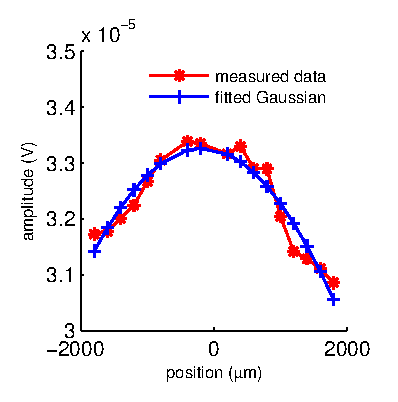
\includegraphics[scale=1]{./Graph/eps/channel3fig.eps}
	\end{center}
	\caption{Amplitude of the envelope of the signal recorded from an electrode at the origin as the source was moved.}
	\label{fig:Ch3}
\end{figure}

\bibliographystyle{plain}
\bibliography{}
\end{document}
